\section{Notes}

\begin{definition}
    The \vocab{locus} (plural: loci) of a variable point is the path traced out by the point under certain conditions.
\end{definition}

\subsection{Standard Loci}

\begin{fact}[Circle]
    For $\abs{z-a} = r$, with $P$ representing the complex number $z$ and $A$ representing the fixed complex number $a$ and $r > 0$, the locus of $P$ is a circle with centre $A$ and radius $r$.

    \begin{center}\tikzsetnextfilename{345}
        \begin{tikzpicture}[trim axis left, trim axis right]
            \begin{axis}[
                domain = 0:10,
                samples = 101,
                axis y line=middle,
                axis x line=middle,
                xtick = \empty,
                ytick = \empty,
                xmax=11.5,
                xmin=-5.5,
                ymin=-4,
                ymax=11,
                xlabel = {$\Re$},
                ylabel = {$\Im$},
                legend cell align={left},
                legend pos=outer north east,
                legend style={fill=none},
                after end axis/.code={
                    \path (axis cs:0,0) 
                        node [anchor=north east] {$O$};
                    }
                ]
    
                \coordinate (O) at (0, 0);
                \coordinate[label=above:$A$] (C) at (3, 4);

                \fill (C) circle[radius=2.5pt];

                \draw[<->] (O) -- (C);

                \node[anchor=west] at (1.7, 2) {$r$};

                \draw[plotRed] (C) circle[radius=5];
                
                \addlegendimage{no markers, plotRed}
                \addlegendentry{locus of $P$};
            \end{axis}
        \end{tikzpicture}
    \end{center}
\end{fact}

\begin{fact}[Perpendicular Bisector]
    For $\abs{z - a} = \abs{z - b}$, with $P$ representing the complex number $z$, points $A$ and $B$ representing the fixed complex numbers $a$ and $b$ respectively, the locus of $P$ is the perpendicular bisector of the line segment joining $A$ and $B$.

    \begin{center}\tikzsetnextfilename{346}
        \begin{tikzpicture}[trim axis left, trim axis right]
            \begin{axis}[
                domain = -10:10,
                samples = 101,
                axis y line=middle,
                axis x line=middle,
                xtick = {-2},
                ytick = {1},
                yticklabels = {},
                xticklabels = {$B$},
                xmax=2,
                xmin=-3,
                ymin=-2,
                ymax=2,
                xlabel = {$\Re$},
                ylabel = {$\Im$},
                legend cell align={left},
                legend pos=outer north east,
                legend style={fill=none},
                after end axis/.code={
                    \path (axis cs:0,0) 
                        node [anchor=north west] {$O$};
                    }
                ]
    
                \coordinate (Z1) at (-2, 0);
                \coordinate (Z2) at (0, 1);
                \coordinate (O) at (0, 0);

                \draw[dotted] (Z1) -- (Z2);

                \addplot[plotRed] {-2*x - 1.5};
        
                \fill (Z1) circle[radius=2.5pt];
                \fill (Z2) circle[radius=2.5pt];

                \addlegendentry{locus of $P$};

                \coordinate (Z3) at (0, -1.5);
                \coordinate (Z4) at (-1, 0.5);
                \draw pic [draw, angle radius=3mm, ""] {right angle =  Z3--Z4--Z2};

                \draw ($(-1.5, 0.25)!0.2cm!270:(Z1)$) -- ($(-1.5, 0.25)!0.2cm!90:(Z1)$);
                \draw ($(-0.5, 0.75)!0.2cm!270:(Z1)$) -- ($(-0.5, 0.75)!0.2cm!90:(Z1)$);

                \node[anchor=west] at (Z2) {$A$};
            \end{axis}
        \end{tikzpicture}
    \end{center}
\end{fact}

\begin{fact}[Half-Line]
    For $\arg{z - a} = \t$, with $P$ representing the complex number $z$ and point $A$ representing the fixed complex number $a$, the locus of $P$ is the half-line starting from $A$ (excluding this point) and inclined at a directed angle $\t$ to the positive real axis.

    \begin{center}\tikzsetnextfilename{347}
        \begin{tikzpicture}[trim axis left, trim axis right]
            \begin{axis}[
                domain = -2:3,
                samples = 101,
                axis y line=middle,
                axis x line=middle,
                xtick = \empty,
                ytick = \empty,
                xmax=2,
                xmin=-3,
                ymin=-2,
                ymax=2,
                xlabel = {$\Re$},
                ylabel = {$\Im$},
                legend cell align={left},
                legend pos=outer north east,
                legend style={fill=none},
                after end axis/.code={
                    \path (axis cs:0,0) 
                        node [anchor=north west] {$O$};
                    }
                ]
    
                \coordinate[label=above:$A$] (Z1) at (-2, 1);
                \coordinate (Z2) at (0, 1);
                \coordinate (O) at (0, 0);

                \draw[dotted] (Z1) -- (Z2);

                \addplot[plotRed] {-x - 1};
        
                \draw (Z1) circle[radius=2.5pt];

                \addlegendentry{locus of $P$};

                \coordinate (Z3) at (0, -1);
                \draw pic [draw, angle radius=12mm, "$\t$"] {angle =  Z3--Z1--Z2};
            \end{axis}
        \end{tikzpicture}
    \end{center}
\end{fact}

\subsection{Non-Standard Loci}

When sketching non-standard loci, one useful technique is to write the equation in Cartesian form, i.e. letting $z = x + \i y$, $x, y \in \RR$.

\begin{example}
    Let $P$ be the point representing the complex number $z$, where $z$ satsifies the equation $\Re z + 2 \Im z = 2$. We begin by writing $z$ in Cartesian form, i.e. $z = x + \i y$, $x, y \in \RR$. Substituting this into the equation, we have $x + 2y = 2$. Thus, the locus of $P$ is given by the equation $x + 2y = 2$.
\end{example}

\subsection{Loci and Inequalities}

To illustrate the general procedure of finding the locus of an inequality, we use $\abs{z - (3 + 4\i)} < 5$ as an example. We begin by considering the equality case. As we have seen above, $\abs{z - (3 + 4\i)} = 5$ corresponds to a circle centred at $(3, 4)$ with radius 5. This is the ``boundary'' of our locus.

\begin{center}\tikzsetnextfilename{348}
    \begin{tikzpicture}[trim axis left, trim axis right]
        \begin{axis}[
            domain = 0:10,
            samples = 101,
            axis y line=middle,
            axis x line=middle,
            xtick = \empty,
            ytick = \empty,
            xmax=11.5,
            xmin=-5.5,
            ymin=-4,
            ymax=11,
            xlabel = {$\Re$},
            ylabel = {$\Im$},
            legend cell align={left},
            legend pos=outer north east,
            legend style={fill=none},
            after end axis/.code={
                \path (axis cs:0,0) 
                    node [anchor=north east] {$O$};
                }
            ]

            \coordinate (O) at (0, 0);
            \coordinate[label=above:$A$] (C) at (3, 4);

            \fill (C) circle[radius=2.5pt];

            \draw[<->] (O) -- (C);

            \node[anchor=west] at (1.7, 2) {$r$};

            \draw[dashed] (C) circle[radius=5];
            
            \addlegendimage{no markers, black}
            \addlegendentry{boundary};
        \end{axis}
    \end{tikzpicture}
\end{center}

Notice that the circle is dashed as the inequality is strict; if the inequality was not strict, i.e. $\abs{z - (3 + 4\i)} \leq 5$, the circle would be drawn with a solid line.

Now, observe that the complex plane has been split into two parts: the interior and exterior of the circle. To determine which region satisfies our inequality, we simply test a complex number in each region.
\begin{itemize}
    \item Since $3 + 4\i$ is in the interior of the circle, and $\abs{(3 + 4\i) - (3 + 4\i)} = 0 < 5$, the interior of the circle satisfies the inequality.
    \item Since $10 + 4\i$ is in the exterior of the circle, and $\abs{(10 + 4\i) - (3 + 4\i)} = 7 > 5$, the exterior of the circle does not satisfy the inequality.
\end{itemize}

We thus conclude that the locus of $\abs{z - (3 + 4\i)} < 5$ is the interior region of the circle, as shaded below:

\begin{center}\tikzsetnextfilename{349}
    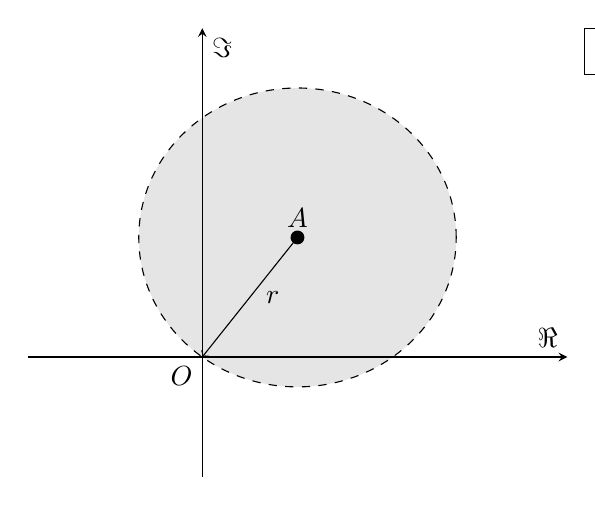
\begin{tikzpicture}[trim axis left, trim axis right]
        \pgfdeclarelayer{pre main}
        \pgfsetlayers{pre main,main}
        \begin{axis}[
            axis on top,
            domain = 0:10,
            samples = 101,
            axis y line=middle,
            axis x line=middle,
            xtick = \empty,
            ytick = \empty,
            xmax=11.5,
            xmin=-5.5,
            ymin=-4,
            ymax=11,
            xlabel = {$\Re$},
            ylabel = {$\Im$},
            legend cell align={left},
            legend pos=outer north east,
            legend style={fill=none},
            after end axis/.code={
                \path (axis cs:0,0) 
                    node [anchor=north east] {$O$};
                }
            ]

            \coordinate (O) at (0, 0);
            \coordinate[label=above:$A$] (C) at (3, 4);

            \pgfonlayer{pre main}
                \fill[black!10] (C) circle[radius=5];
            \endpgfonlayer

            \fill (C) circle[radius=2.5pt];

            \draw[<->] (O) -- (C);

            \node[anchor=west] at (1.7, 2) {$r$};

            \draw[dashed] (C) circle[radius=5];           

            \addlegendimage{line legend, black!10, line width=5pt}
            \addlegendentry{required locus};
        \end{axis}
    \end{tikzpicture}
\end{center}

\subsection{Further Use of the Argand Diagram}

Many interesting and varied problems involving complex numbers can be solved simply using an Argand diagram. For instance, one may ask what the range of $\arg z$ is, given that $z$ satisfies some other constraint, e.g. $\abs{z - \i} = 1$. Given how diverse these problems may be, there is no general approach to solving them. However, there are several tips that one should keep in mind when doing these problems:
\begin{itemize}
    \item Think geometrically! Draw out the given constraints on an Argand diagram. Most of the time, the given constraints are simply the three standard loci above (circles, perpendicular bisector and half-lines).
    \item When working with circles and an external point, drawing tangents and diameters may help. This allows one to use properties of circles (e.g. tangents are perpendicular to the radius).
    \item Keep an eye out for symmetry or similar figures.
\end{itemize}